%!TEX root = ../Report.tex
***Explain pattern implemented, (similar to OpenMP (Loop scheduling) and skepu, add differences to blackbourn's work) details of library (Controller etc), and how it may be used in a real system***

In this chapter, we will discuss the design of the system created to investigate this problem, and detail how such a system could be extended for the future.



\section{System description}

The ideas described in the background section are combined to produce a skeleton programming library with plasticity and contention aware scheduling. To keep it simple, we build the system incrementally, starting with a single parallel pattern, later adding plasticity and contention aware scheduling. 



\subsection{Skeleton Foundation}

As discussed in the background section, one of the key ideas behind the project is that of skeleton programming, using predefined patterns to aid the programmer. The first pattern implemented is the map array pattern, with further patterns left for possible future work. Map-array is similar to the map pattern, in that it applies a given user function to each element in a list, however map-array also allows the function to access a user provided array. This was chosen as the map pattern is likely the most well known pattern and certainly one of the most useful, and map-array provides further functionality on top of this. It also provides a good basis for developing further patterns, and it also allows complex testing, which will be covered in the evaluation section of this report.



\subsection{Adding Plasticity}

To implement plasticity, we add the ability to vary three key aspects of the implementation of map-array:

\begin{itemize}
	\item Thread count - The number of threads we split the tasks between
	\item Thread pinnings - The particular CPU core each thread runs on
	\item Schedule - How to divide tasks between threads
\end{itemize}

The thread count and pinnings are self explanatory. The schedule however requires some explanation.

The most basic method to divide the tasks is to give an equal amount to each thread. This is fine if the complexity of the tasks is uniform, but if it is skewed, the amount of computation to be done by each thread is imbalanced. This is illustrated in figure \ref{fig:unoptimized_schedule}. This is because we have idle cores during computation, which is a wasted resource in a multi-threaded execution. However, if we allocate the tasks differently, we can obtain better performance, as illustrated in figure \ref{fig:optimized_schedule}.

So load balancing a workload is critical to performance in such a multi-threaded application. However, optimizing the task distribution in this manner is non trivial, and it depends upon the computation to be done as well as the number of threads and other resources available at runtime.

A solution to this problem is to provide many different task distributions, and let the user pick or the machine select which distribution to use. These are called schedules, and some common ones are:

\begin{itemize}
	\item Static - An equal allocation to all threads
	\item Dynamic individual - Each thread retrieves one task at a time, and once completed, it goes back for more
	\item Dynamic chunks - Each thread retrieves N tasks at a time, and once completed, it goes back for more
	\item Tapered - Each thread starts by retrieving N tasks at a time, and as the computation continues, it retrieves less and less
\end{itemize}

Thread count and schedule were chosen as they seem the most critical to performance, and thread pinnings was added as this is was investigated in the LIRA paper (cite LIRA) as a factor contention aware scheduling could exploit.

Once we have added plasticity, we can experiment with the specifics of an implementation, and see how they affect the performance of the system. This would be the use case of utilizing our library with no other program running, (So no contention aware scheduling), and we can explore how we can adapt the program using plasticity at runtime in this case. We may be able to improve performance even under these conditions, depending upon the configuration of the the machine (e.g., is there more CPU cores available) and the problem (e.g. do we have many small tasks or few large tasks.) 



\begin{figure}
	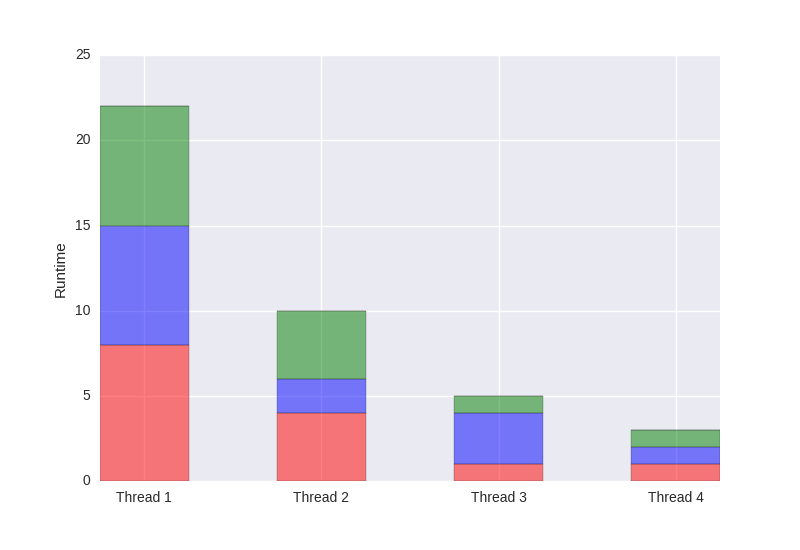
\includegraphics[width=\textwidth]{graphics/unoptimized_schedule.png}
	\caption{A worst case scenario of a static schedule assigning each thread an equal number of tasks}
	\label{fig:unoptimized_schedule}
\end{figure}

\begin{figure}
	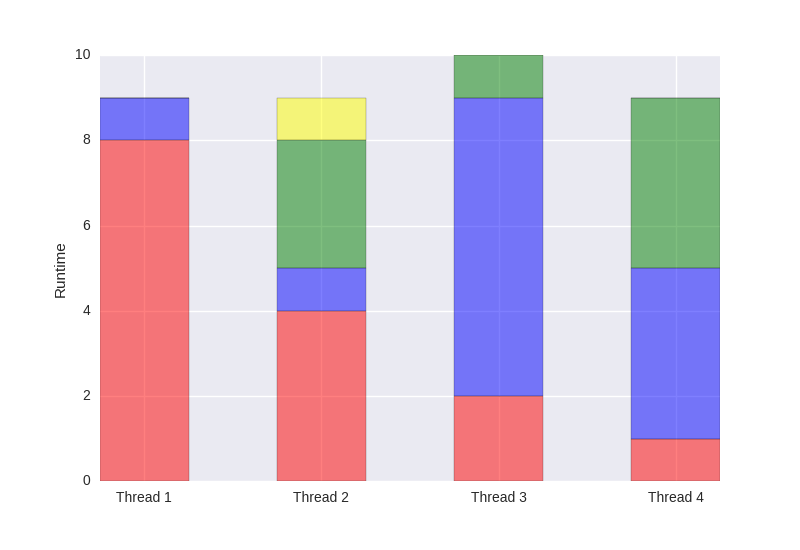
\includegraphics[width=\textwidth]{graphics/optimized_schedule.png}
	\caption{An optimized version of figure \ref{fig:unoptimized_schedule}, notice that thread 2 has four tasks, but the total runtime is substantially less}
	\label{fig:optimized_schedule}
\end{figure}



\subsection{Contention Aware Scheduling}

To add contention aware scheduling, we need multiple instances of our library to be able to collaborate, and adapt their behaviour accordingly. To do this, we use a separate controller application, with which all instances of our program can communicate. This provides a single known point of contact, and a designated thread for computing program parameters with respect to all aspects of the system. An example of how our programs and the controller program communicate is shown in figure 

Once our programs can communicate, and we can control each aspect of them, we can implement contention aware scheduling. (***Is changing something like the schedule still scheduling?***) For testing purposes, we simply program a set of predefined actions for the controller to take, in order to manually control what each implementation does, as we are only investigating if this can be taken further. We leave implementing some algorithm for automatic parameter tuning for future work.

***Refine from here***

As an example of how this would work in practice is in figure \ref{fig:controller_flowchart}.

Now that we have contention aware scheduling, we can experiment with multiple programs running on a system at once. An example of how plastic programming and contention aware scheduling is given in figure \ref{fig:plastic_contention_aware_scheduling}



\begin{figure}
	\includegraphics[width=0.8\textwidth]{graphics/controller_flowchart.png}
	\caption{How applications communicate with the controller ***Not too happy with this diagram, could be clearer. Also, pretty huge.***}
	\label{fig:controller_flowchart}
\end{figure}

\begin{figure}
	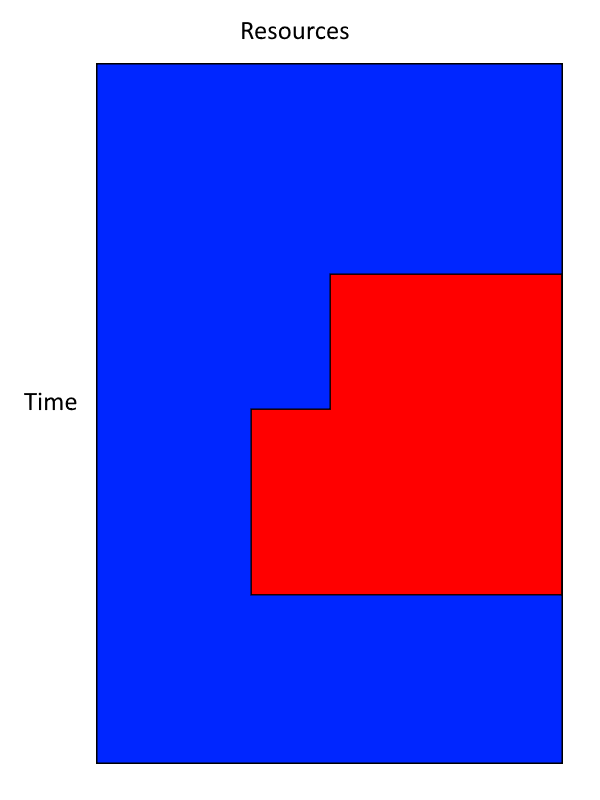
\includegraphics[width=0.8\textwidth]{graphics/placeholder_plastic_contention_aware_scheduling.png}
	\caption{***Place-holder graph for plastic contention aware scheduling***}
	\label{fig:plastic_contention_aware_scheduling}
\end{figure}



\subsection{Evaluation}

To properly evaluate the outcome of this project, we need some way of testing the libraries performance. To this end, we implemented a placebo program which evaluates the library with a synthetic workload, collecting and recording metrics detailing the libraries performance with different parameters.  

We also need points of comparison in terms of performance. So, in addition to our placebo program, we also implement an equivalent sequential and an OpenMP version, in which we can vary similar parameters and produce comparable statistics. 

(*** If complete, add that they utilize the same testing framework)

(***NOTE - designing for future applications has been moved to the future work chapter***)